\documentclass[]{article}
\usepackage{lmodern}
\usepackage{amssymb,amsmath}
\usepackage{ifxetex,ifluatex}
\usepackage{fixltx2e} % provides \textsubscript
\ifnum 0\ifxetex 1\fi\ifluatex 1\fi=0 % if pdftex
  \usepackage[T1]{fontenc}
  \usepackage[utf8]{inputenc}
\else % if luatex or xelatex
  \ifxetex
    \usepackage{mathspec}
  \else
    \usepackage{fontspec}
  \fi
  \defaultfontfeatures{Ligatures=TeX,Scale=MatchLowercase}
\fi
% use upquote if available, for straight quotes in verbatim environments
\IfFileExists{upquote.sty}{\usepackage{upquote}}{}
% use microtype if available
\IfFileExists{microtype.sty}{%
\usepackage{microtype}
\UseMicrotypeSet[protrusion]{basicmath} % disable protrusion for tt fonts
}{}
\usepackage[margin=1in]{geometry}
\usepackage{hyperref}
\hypersetup{unicode=true,
            pdftitle={Half the Thrill is in the Chase},
            pdfborder={0 0 0},
            breaklinks=true}
\urlstyle{same}  % don't use monospace font for urls
\usepackage{color}
\usepackage{fancyvrb}
\newcommand{\VerbBar}{|}
\newcommand{\VERB}{\Verb[commandchars=\\\{\}]}
\DefineVerbatimEnvironment{Highlighting}{Verbatim}{commandchars=\\\{\}}
% Add ',fontsize=\small' for more characters per line
\usepackage{framed}
\definecolor{shadecolor}{RGB}{248,248,248}
\newenvironment{Shaded}{\begin{snugshade}}{\end{snugshade}}
\newcommand{\AlertTok}[1]{\textcolor[rgb]{0.94,0.16,0.16}{#1}}
\newcommand{\AnnotationTok}[1]{\textcolor[rgb]{0.56,0.35,0.01}{\textbf{\textit{#1}}}}
\newcommand{\AttributeTok}[1]{\textcolor[rgb]{0.77,0.63,0.00}{#1}}
\newcommand{\BaseNTok}[1]{\textcolor[rgb]{0.00,0.00,0.81}{#1}}
\newcommand{\BuiltInTok}[1]{#1}
\newcommand{\CharTok}[1]{\textcolor[rgb]{0.31,0.60,0.02}{#1}}
\newcommand{\CommentTok}[1]{\textcolor[rgb]{0.56,0.35,0.01}{\textit{#1}}}
\newcommand{\CommentVarTok}[1]{\textcolor[rgb]{0.56,0.35,0.01}{\textbf{\textit{#1}}}}
\newcommand{\ConstantTok}[1]{\textcolor[rgb]{0.00,0.00,0.00}{#1}}
\newcommand{\ControlFlowTok}[1]{\textcolor[rgb]{0.13,0.29,0.53}{\textbf{#1}}}
\newcommand{\DataTypeTok}[1]{\textcolor[rgb]{0.13,0.29,0.53}{#1}}
\newcommand{\DecValTok}[1]{\textcolor[rgb]{0.00,0.00,0.81}{#1}}
\newcommand{\DocumentationTok}[1]{\textcolor[rgb]{0.56,0.35,0.01}{\textbf{\textit{#1}}}}
\newcommand{\ErrorTok}[1]{\textcolor[rgb]{0.64,0.00,0.00}{\textbf{#1}}}
\newcommand{\ExtensionTok}[1]{#1}
\newcommand{\FloatTok}[1]{\textcolor[rgb]{0.00,0.00,0.81}{#1}}
\newcommand{\FunctionTok}[1]{\textcolor[rgb]{0.00,0.00,0.00}{#1}}
\newcommand{\ImportTok}[1]{#1}
\newcommand{\InformationTok}[1]{\textcolor[rgb]{0.56,0.35,0.01}{\textbf{\textit{#1}}}}
\newcommand{\KeywordTok}[1]{\textcolor[rgb]{0.13,0.29,0.53}{\textbf{#1}}}
\newcommand{\NormalTok}[1]{#1}
\newcommand{\OperatorTok}[1]{\textcolor[rgb]{0.81,0.36,0.00}{\textbf{#1}}}
\newcommand{\OtherTok}[1]{\textcolor[rgb]{0.56,0.35,0.01}{#1}}
\newcommand{\PreprocessorTok}[1]{\textcolor[rgb]{0.56,0.35,0.01}{\textit{#1}}}
\newcommand{\RegionMarkerTok}[1]{#1}
\newcommand{\SpecialCharTok}[1]{\textcolor[rgb]{0.00,0.00,0.00}{#1}}
\newcommand{\SpecialStringTok}[1]{\textcolor[rgb]{0.31,0.60,0.02}{#1}}
\newcommand{\StringTok}[1]{\textcolor[rgb]{0.31,0.60,0.02}{#1}}
\newcommand{\VariableTok}[1]{\textcolor[rgb]{0.00,0.00,0.00}{#1}}
\newcommand{\VerbatimStringTok}[1]{\textcolor[rgb]{0.31,0.60,0.02}{#1}}
\newcommand{\WarningTok}[1]{\textcolor[rgb]{0.56,0.35,0.01}{\textbf{\textit{#1}}}}
\usepackage{graphicx,grffile}
\makeatletter
\def\maxwidth{\ifdim\Gin@nat@width>\linewidth\linewidth\else\Gin@nat@width\fi}
\def\maxheight{\ifdim\Gin@nat@height>\textheight\textheight\else\Gin@nat@height\fi}
\makeatother
% Scale images if necessary, so that they will not overflow the page
% margins by default, and it is still possible to overwrite the defaults
% using explicit options in \includegraphics[width, height, ...]{}
\setkeys{Gin}{width=\maxwidth,height=\maxheight,keepaspectratio}
\IfFileExists{parskip.sty}{%
\usepackage{parskip}
}{% else
\setlength{\parindent}{0pt}
\setlength{\parskip}{6pt plus 2pt minus 1pt}
}
\setlength{\emergencystretch}{3em}  % prevent overfull lines
\providecommand{\tightlist}{%
  \setlength{\itemsep}{0pt}\setlength{\parskip}{0pt}}
\setcounter{secnumdepth}{0}
% Redefines (sub)paragraphs to behave more like sections
\ifx\paragraph\undefined\else
\let\oldparagraph\paragraph
\renewcommand{\paragraph}[1]{\oldparagraph{#1}\mbox{}}
\fi
\ifx\subparagraph\undefined\else
\let\oldsubparagraph\subparagraph
\renewcommand{\subparagraph}[1]{\oldsubparagraph{#1}\mbox{}}
\fi

%%% Use protect on footnotes to avoid problems with footnotes in titles
\let\rmarkdownfootnote\footnote%
\def\footnote{\protect\rmarkdownfootnote}

%%% Change title format to be more compact
\usepackage{titling}

% Create subtitle command for use in maketitle
\providecommand{\subtitle}[1]{
  \posttitle{
    \begin{center}\large#1\end{center}
    }
}

\setlength{\droptitle}{-2em}

  \title{Half the Thrill is in the Chase}
    \pretitle{\vspace{\droptitle}\centering\huge}
  \posttitle{\par}
    \author{}
    \preauthor{}\postauthor{}
      \predate{\centering\large\emph}
  \postdate{\par}
    \date{10/24/2019}


\begin{document}
\maketitle

\begin{Shaded}
\begin{Highlighting}[]
\CommentTok{# This function takes in a data frame of characteristics and simulates nreps standard deviations}
\NormalTok{sd_samp <-}\StringTok{ }\ControlFlowTok{function}\NormalTok{(df, reps) \{}
  \CommentTok{# Number of people in each cell}
\NormalTok{  nper <-}\StringTok{ }\KeywordTok{as.numeric}\NormalTok{(df[}\DecValTok{1}\NormalTok{, }\StringTok{"n_per"}\NormalTok{])}
  \CommentTok{# Minimum score on the scale}
\NormalTok{  minscore <-}\StringTok{ }\KeywordTok{as.numeric}\NormalTok{(df[}\DecValTok{1}\NormalTok{, }\StringTok{"min_score"}\NormalTok{])}
  \CommentTok{# Maximum score on the scale}
\NormalTok{  maxscore <-}\StringTok{ }\KeywordTok{as.numeric}\NormalTok{(df[}\DecValTok{1}\NormalTok{, }\StringTok{"max_score"}\NormalTok{])}
  \CommentTok{# mean observed}
\NormalTok{  mean <-}\StringTok{ }\KeywordTok{as.numeric}\NormalTok{(df[}\DecValTok{1}\NormalTok{, }\StringTok{"mean"}\NormalTok{])}
  \CommentTok{# pooled sd }
\NormalTok{  pooledsd <-}\StringTok{ }\KeywordTok{as.numeric}\NormalTok{(df[}\DecValTok{1}\NormalTok{, }\StringTok{"pooled_sd_obs"}\NormalTok{])}
  
  \CommentTok{# Simulate SDs}
  \CommentTok{# }\AlertTok{NOTE}\CommentTok{: I'm using a truncated normal distribution because they use a 1-7 scale}
\NormalTok{  reps <-}\StringTok{ }\KeywordTok{replicate}\NormalTok{(reps,}
                    \KeywordTok{sd}\NormalTok{(}\KeywordTok{rtruncnorm}\NormalTok{(nper, }\DataTypeTok{a =}\NormalTok{ minscore, }\DataTypeTok{b =}\NormalTok{ maxscore, }\DataTypeTok{mean =}\NormalTok{ mean, }
                                  \DataTypeTok{sd =}\NormalTok{ pooledsd))) }
\NormalTok{  reps <-}\StringTok{ }\KeywordTok{as.data.frame}\NormalTok{(reps)}
  
  \KeywordTok{names}\NormalTok{(reps) <-}\StringTok{ "sd_rep"}
  
\NormalTok{  reps}
\NormalTok{\}}
\end{Highlighting}
\end{Shaded}

\begin{Shaded}
\begin{Highlighting}[]
\CommentTok{# Add in the number of participants per cell and the standard deviation to table 1}
\NormalTok{tbl1 <-}\StringTok{ }\NormalTok{tbl1 }\OperatorTok
\StringTok{  }\KeywordTok{mutate}\NormalTok{(}\DataTypeTok{n_per =} \DecValTok{11}\NormalTok{,}
         \DataTypeTok{sd =}\NormalTok{ se }\OperatorTok{*}\StringTok{ }\KeywordTok{sqrt}\NormalTok{(n_per)) }\OperatorTok
\StringTok{  }\KeywordTok{arrange}\NormalTok{(variable) }

\CommentTok{# create sd_sd and mean_sd for each variable in the study}
\NormalTok{tbl1_sum <-}\StringTok{ }\NormalTok{tbl1 }\OperatorTok
\StringTok{  }\KeywordTok{group_by}\NormalTok{(variable) }\OperatorTok
\StringTok{  }\KeywordTok{summarise}\NormalTok{(}\DataTypeTok{sd_sd_obs =} \KeywordTok{sd}\NormalTok{(sd),}
            \DataTypeTok{pooled_sd_obs =} \KeywordTok{mean}\NormalTok{(sd),}
            \DataTypeTok{mean_n_obs =} \KeywordTok{mean}\NormalTok{(n_per),}
            \DataTypeTok{se_sds_obs =}\NormalTok{ pooled_sd_obs}\OperatorTok{/}\NormalTok{(}\KeywordTok{sqrt}\NormalTok{(}\DecValTok{2}\OperatorTok{*}\NormalTok{mean_n_obs)),}
            \DataTypeTok{psi_obs =}\NormalTok{ sd_sd_obs }\OperatorTok{/}\StringTok{ }\NormalTok{se_sds_obs)}

\CommentTok{# merge dataframes (need this for the simulation)}
\NormalTok{tbl1 <-}\StringTok{ }\KeywordTok{merge}\NormalTok{(tbl1, tbl1_sum)}
\end{Highlighting}
\end{Shaded}

\begin{Shaded}
\begin{Highlighting}[]
\NormalTok{reps <-}\StringTok{ }\DecValTok{100000}

\CommentTok{# simulate SDs}
\NormalTok{tbl1_reps <-}\StringTok{ }\NormalTok{tbl1 }\OperatorTok
\StringTok{  }\KeywordTok{group_by}\NormalTok{(variable, manip) }\OperatorTok
\StringTok{  }\KeywordTok{do}\NormalTok{(}\KeywordTok{sd_samp}\NormalTok{(}\DataTypeTok{df =}\NormalTok{ ., }\DataTypeTok{reps =}\NormalTok{ reps))}

\CommentTok{# add in the replication number}
\NormalTok{tbl1_reps <-}\StringTok{ }\NormalTok{tbl1_reps }\OperatorTok
\StringTok{  }\KeywordTok{group_by}\NormalTok{(variable, manip) }\OperatorTok
\StringTok{  }\KeywordTok{mutate}\NormalTok{(}\DataTypeTok{n_rep =} \DecValTok{1}\OperatorTok{:}\NormalTok{reps) }

\CommentTok{# Summarized simulated data}
\NormalTok{tbl1_reps_sum <-}\StringTok{ }\NormalTok{tbl1_reps }\OperatorTok\StringTok{ }
\StringTok{  }\KeywordTok{group_by}\NormalTok{(variable, n_rep) }\OperatorTok
\StringTok{  }\KeywordTok{summarise}\NormalTok{(}\DataTypeTok{sd_sd_sim =} \KeywordTok{sd}\NormalTok{(sd_rep),}
            \DataTypeTok{pooled_sd_sim =} \KeywordTok{mean}\NormalTok{(sd_rep)) }\OperatorTok
\StringTok{    }\CommentTok{# get the simulated standard deviations and psi's}
\StringTok{  }\KeywordTok{mutate}\NormalTok{(}\DataTypeTok{se_sd_sim =}\NormalTok{ pooled_sd_sim}\OperatorTok{/}\NormalTok{(}\KeywordTok{sqrt}\NormalTok{(}\DecValTok{2} \OperatorTok{*}\StringTok{ }\DecValTok{11}\NormalTok{)),}
         \DataTypeTok{psi_sim =}\NormalTok{ sd_sd_sim}\OperatorTok{/}\NormalTok{se_sd_sim)}

\CommentTok{# merge simulated data with empirical data}
\NormalTok{tbl1_reps_sum <-}\StringTok{ }\NormalTok{tbl1_reps_sum }\OperatorTok\StringTok{ }
\StringTok{  }\KeywordTok{left_join}\NormalTok{(tbl1_sum)}
\end{Highlighting}
\end{Shaded}

\begin{verbatim}
## Joining, by = "variable"
\end{verbatim}

\begin{Shaded}
\begin{Highlighting}[]
\CommentTok{# compare the number of observed sds that are larger than the simulated sds}
\NormalTok{tbl1_reps_sum <-}\StringTok{ }\NormalTok{tbl1_reps_sum }\OperatorTok
\StringTok{  }\KeywordTok{mutate}\NormalTok{(}\DataTypeTok{obs_gt_sim =} \KeywordTok{ifelse}\NormalTok{(sd_sd_obs }\OperatorTok{>=}\StringTok{ }\NormalTok{sd_sd_sim, }\OtherTok{TRUE}\NormalTok{, }\OtherTok{FALSE}\NormalTok{))}
\end{Highlighting}
\end{Shaded}

\hypertarget{sd-similarity}{%
\section{SD Similarity}\label{sd-similarity}}

\hypertarget{within-measures}{%
\subsection{Within measures}\label{within-measures}}

Density plots of the simulated standard deviations for each of the
measures reported in Table 1 of Labroo and Nielsen. Vertical Lines
represent the observed standard deviation of standard deviations. Note
that the observed standard deviations are all unlikely

\begin{Shaded}
\begin{Highlighting}[]
\CommentTok{# plot the histograms}
\KeywordTok{ggplot}\NormalTok{(tbl1_reps_sum, }\KeywordTok{aes}\NormalTok{(}\DataTypeTok{x =}\NormalTok{ sd_sd_sim)) }\OperatorTok{+}
\StringTok{  }\KeywordTok{geom_density}\NormalTok{() }\OperatorTok{+}
\StringTok{  }\KeywordTok{geom_vline}\NormalTok{(}\KeywordTok{aes}\NormalTok{(}\DataTypeTok{xintercept =}\NormalTok{ sd_sd_obs)) }\OperatorTok{+}
\StringTok{  }\KeywordTok{facet_grid}\NormalTok{(variable }\OperatorTok{~}\StringTok{ }\NormalTok{.) }\OperatorTok{+}
\StringTok{  }\KeywordTok{theme_classic}\NormalTok{()}
\end{Highlighting}
\end{Shaded}

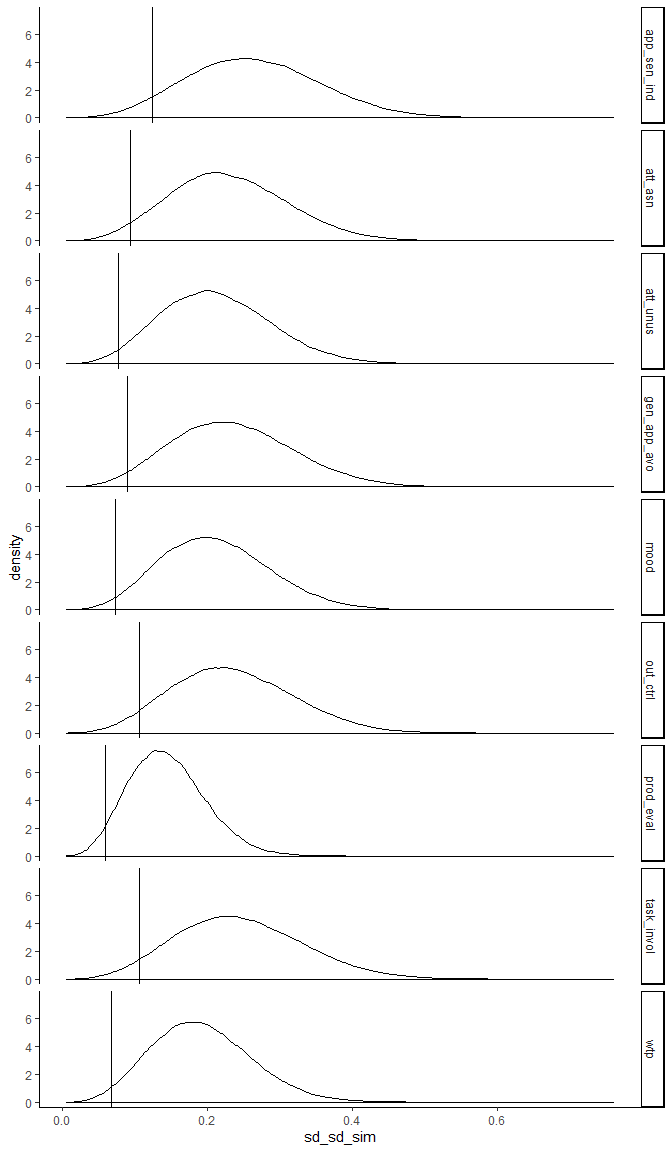
\includegraphics{Labroo-Nielsen-analysis_files/figure-latex/Plot-1.pdf}

\hypertarget{combined-measures}{%
\subsection{Combined measures}\label{combined-measures}}

Now combining the standard deviations across measures.\\
From Simonsohn 2013 pg. 1878

\begin{quote}
Before aggregating, however, I had to get around the problem that the
studies differed in scale (e.g., grams of hot sauce vs. number of fish)
and sample size (n = 15 vs.~n = 20). An easy way to do this was to
divide the standard deviation of the standard deviations by the standard
error of the (pooled) standard deviation. This yielded an intuitive
measure of deviation the number of standard errors by which the standard
deviations differed within a given study. I refer to this number as Ψ
\end{quote}

NOTE: Whereas Simonsohn (2013) combined dependent variables across
multiple studies, I am combining across multiple measures within a
single study. This should not be an issue unless we believe that there
is a correlation between standard deviations.

\begin{Shaded}
\begin{Highlighting}[]
\NormalTok{sim_meanpsi <-}\StringTok{ }\NormalTok{tbl1_reps_sum }\OperatorTok
\StringTok{  }\KeywordTok{group_by}\NormalTok{(n_rep) }\OperatorTok
\StringTok{  }\CommentTok{# get mean psi for each replication}
\StringTok{  }\KeywordTok{summarise}\NormalTok{(}\DataTypeTok{mean_psi_sim =} \KeywordTok{mean}\NormalTok{(psi_sim),}
            \DataTypeTok{psi_obs =}\NormalTok{ psi_obs[}\DecValTok{1}\NormalTok{]) }\OperatorTok
\StringTok{  }\CommentTok{# get the number of simulated SD's which are larger than the observed}
\StringTok{  }\KeywordTok{mutate}\NormalTok{(}\DataTypeTok{simpsi_gt_stupsi =} \KeywordTok{ifelse}\NormalTok{(mean_psi_sim }\OperatorTok{>}\StringTok{ }\NormalTok{psi_obs, }\OtherTok{TRUE}\NormalTok{, }\OtherTok{FALSE}\NormalTok{))}
\end{Highlighting}
\end{Shaded}

Of the simulated standard deviations, 100000 of the \ensuremath{10^{5}}
had higher \(\psi\) values than the observed \(\psi\) value. That is,
the combined measure of the variability of standard deviation was higher
for every simulation than the observed data.

Density plot of the simulated \(\psi\) values. Note that the observed
\(\psi\) is below any of the simulated \(\psi\) values.

\begin{Shaded}
\begin{Highlighting}[]
\NormalTok{sim_meanpsi }\OperatorTok\StringTok{ }
\StringTok{  }\KeywordTok{ggplot}\NormalTok{(}\KeywordTok{aes}\NormalTok{(}\DataTypeTok{x =}\NormalTok{ mean_psi_sim)) }\OperatorTok{+}
\StringTok{  }\KeywordTok{geom_density}\NormalTok{() }\OperatorTok{+}
\StringTok{  }\KeywordTok{geom_vline}\NormalTok{(}\KeywordTok{aes}\NormalTok{(}\DataTypeTok{xintercept =}\NormalTok{ psi_obs)) }\OperatorTok{+}
\StringTok{  }\KeywordTok{theme_classic}\NormalTok{()}
\end{Highlighting}
\end{Shaded}

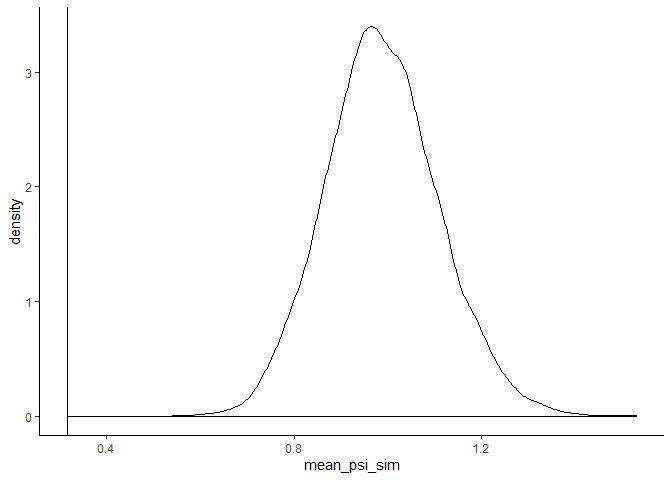
\includegraphics{Labroo-Nielsen-analysis_files/figure-latex/unnamed-chunk-1-1.pdf}

\hypertarget{further-note}{%
\section{Further note}\label{further-note}}

This study is on a similar topic to Sanna et al (2011). Both Sanna and
Nielsen were affiliated with the University of North Carolina.
\url{http://u.arizona.edu/~jesper/Vita.pdf}
\url{https://sites.google.com/view/lawrencejsanna/employment?authuser=0}


\end{document}
